% https://liam0205.me/2014/09/08/latex-introduction/index.html
% \开头的称为控制序列, 影响输出文档的效果, {}内为参数.
% 部分控制序列还有被[]包括的可选参数.
\documentclass[a4paper, 11pt]{article}
% \documentclass和\begin之间为`导言区`, 其中的控制序列一般影响整个输出文档.

% \usepackage{}用来调用宏包.

% 作者, 标题, 日期
% 使用`titling`可修改默认title格式
% http://texdoc.net/texmf-dist/doc/latex/titling/titling.pdf
\usepackage{titling}
\title{}
\author{Jin Dong}
% amsmath宏包提供数学功能.
% 公式分为inline($...$)和display(\[...\])两种模式.
% 若需要对公式编号, 使用equation模式\begin{equation}
\usepackage{amsmath}

\usepackage{tabularx}
\usepackage{caption}
\usepackage{float}

% graphicx宏包的\includegraphics命令用于插入图片
\usepackage{graphicx}

% 使用geometry宏包设置页边距
\usepackage{geometry}
% \geometry{papersize={20cm, 15cm}}
\geometry{left=2cm, right=2cm, top=2cm, bottom=2cm}

% 使用fancyhdr宏包设置页眉页脚
% http://texdoc.net/texmf-dist/doc/latex/fancyhdr/fancyhdr.pdf
\usepackage{fancyhdr}
\pagestyle{fancy}
\lhead{}
\chead{}
\rhead{}
%\lfoot{}
%\cfoot{\thepage}
%\rfoot{}
% 页眉和正文间的横线分割
\renewcommand{\headrulewidth}{0.4pt}
\renewcommand{\headwidth}{\textwidth}
\renewcommand{\footrulewidth}{0.4pt}

% 首行缩进两个中文汉字长度
%\usepackage{indentfirst}
%\setlength{\parindent}{\ccwd}

% 行间距通过setspace宏包调整, 如字号的1.5倍
\usepackage{setspace}
\onehalfspacing

% 段间距, 通过修改长度\parskip的值来调整
\addtolength{\parskip}{.4em}

\newcommand{\newAssignment}[2]{
	\begin{center}
  		\textbf{{\huge #1}}\vspace{5pt} \\
  		{\large #2}\vspace{5pt}
	\end{center}
}
\newcommand{\newQuestion}[1]{\textbf{\Large #1}}
\newcommand{\newPart}[1]{\textbf{\large #1}}
\newcommand{\newImage}[2]{\includegraphics[width = #1\textwidth]{#2}}

\begin{document}
\newAssignment{COMP 512: Performance Analysis Report}{Jin Dong, 260860634; Shiquan Zhang, 260850447}

% \maketitle
% \tableofcontents
% 在文章类article/ctexart中定义了五个控制序列来调整行文组织:
% section\{\}
% subsection\{\}
% subsubsection\{\}
% paragraph\{\}
% subparagraph\{\}

\vspace{-35pt}
\section{Test Bed}
\vspace{-15pt}
     The performance test has two parts: single client and multiple clients. In the multiple client test, we measure the performance with 2, 4, 6 and 8 clients in the system. \par
     In each client, we use 200 $customers$, 200 $flights$ and 100 $locations/cities$. At the preparation phase, we add these $customers$, $flights$, $cars$ and $rooms$ to the server. Then in the test phase, we run 100 iterations with different itineraries. In each itinerary, client sends 9 requests in one transaction: $start$, $queryCustomer$, $queryFlight$, $reserveFlight$, $queryCar$, $reserveCar$, $queryRoom$, $reserveRoom$ and $commit$. In the single RM test, in order to keep the same operation in one transaction, we make 3 $query-reserve$ pair on the $flight$ RM. \par
     We measure the response time of every request in the itinerary and calculate the $average query time$ of 4 queries and $average reserve time$ of 3 reservations. Besides, we also record the time of every transaction/itinerary. When calculating the overall $average time$, we leverage the time in the last 80 iterations to get the stable result. \par
     In the multiple client test, we need to avoid deadlock. We use $(i*8 + clientNum) \% cityNum$ as the index, which can avoid different clients reading and writing the same object at the same time. Additionally, we add a $\pm 1\%$ variation in every transaction time interval.
\vspace{-20pt}
\section{Test Result}
\vspace{-10pt}
\subsection{Single Client Test}
\vspace{-10pt}
      The overall average start time, query time, reserve time and commit time with single RM and multiple RM in single client test is shown in Table 1. The unit of the values is millisecond.
\begin{table}[H]
\centering
\label{tab:Table_1}
\begin{tabular}{| c | c | c | c | c | c |}
	\hline
	/ms & Start Time & Query Time & Reserve Time & Commit Time & Tx Time \\ \hline
	Single RM & 0.31 & 0.533768 & 0.650833 & 0.61 & 5.02 \\ \hline
	Multiple RM & 0.3375 & 0.903125 & 1.0575 & 2.2875 & 9.425 \\ \hline
\end{tabular}
\vspace{-5pt}
\captionof{table}{Response Time of the Single Client Test with Single/Multiple RM}
\end{table}
\vspace{-35pt}
\subsection{Multiple Client Test}
\vspace{-10pt}
      The average transaction time of multiple client test with different transaction rates and different number of clients are shown in Figure 1. Since the minimum time interval between two transactions is 1 ms, the maximum transaction rate varies from 2000 tx/s to 8000 tx/s.
\vspace{-5pt}
\begin{figure}[H]
    \centering
    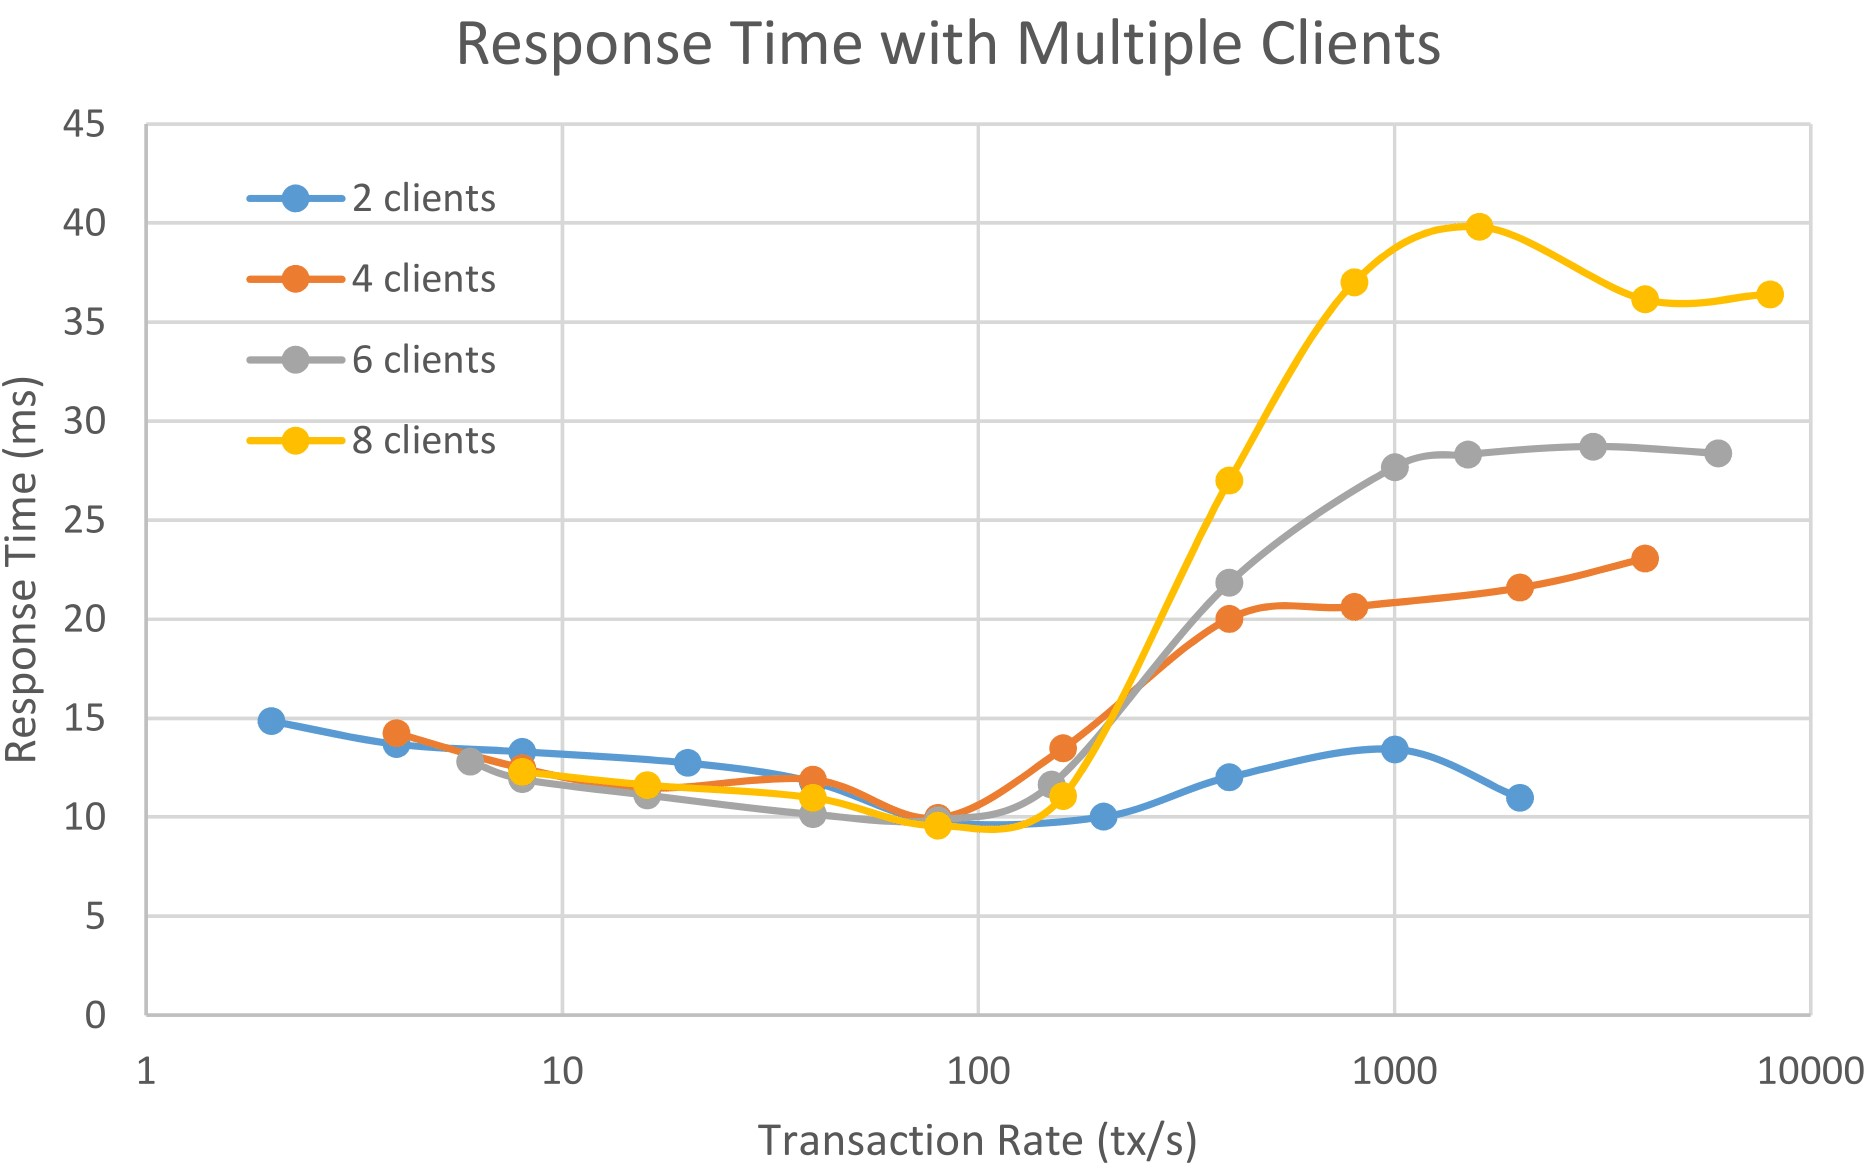
\includegraphics[width=0.6\linewidth]{test_results-1.jpg}
    \vspace{-5pt}
    \caption{Response Time of Multiple Client Test}
    \label{fig:Figure_1}
    \vspace{-10pt}
\end{figure}
\vspace{-10pt}
\section{Performance Analysis}
\vspace{-10pt}
\subsection{Single Client Test}
\vspace{-10pt}
      From Table 1, we can see that the total transaction time is roughly the linear combination of all requests time: $T_{start} + 4\times T_{query} + 3\times T_{reserve} + T_{commit}\approx T_{tx}$. Consider the differece between the query time and reserve time, the reserve operation not only reads the data but also writes new data to item RM and customer RM, thus the difference (around 0.1 ms) is casused by the write operation. \par
      Comparing the response time between single RM and multiple RM, the differences are mainly in query, reservation and commit. In query and reserve, the operations of two types of transactions are different mainly in lock management and saving undo hashmap. In every round of multiple RM test, the query requests have 2 more locks to grant and the reserve requests have 2 more locks to convert and 2 more items to save the undo hashmap. In commit requests, the cost difference is relatively large, since in the multiple RM test, Middleware needs to communicate with 2 more RMs, which costs much more time. Therefore, we can infer that the time is mainly spent in lock management in Middleware when querying, in data writing and undo hashmap saving in RM when reserving, and in communication when committing.
\vspace{-15pt}
\subsection{Multiple Client Test}
\vspace{-10pt}
      From Figure 1, we can see that when the transaction rate is less than 100 tx/s, the response time remains low. When the transaction rate increases to $[100, 1000]$ tx/s, the response time goes up. When the transaction rate is more than 100 tx/s, the system is saturated and the response time remains in a high level. \par
      When the workload is low, the system can handle all the requests from different clients in time, so the average response time is close to that in the single client test. When the workload increases, the server is no longer be able to handle all the transactions in time, so the response time increases. When the workload goes beyond some point around 1000 tx/s, the time interval between transactions is less than the response time, thus the client will continuously send the request and the system is saturated. \par
      Furthermore, if we look into the response time with high workload by time slots, we can see that there are some spikes in the response time, which means that sometime the transactions from all clients are congested in the server at the same time and causing the overall average response time larger than normal case. This may be caused by the data switching between memory and disk in Middleware. \par
      For custom functionality, we also test the system with 2, 4, 6 and 8 clients. The response time with different number of clients are the same when the workload is low and all reach the lowest point at around 100 tx/s. Then all the response time increase until saturated, while the response time with 2 clients increases little. Besides, the saturated response time are roughly linear to the number of clients, because although the transaction rate is the same, the middleware needs to handle more requests at the same time with more clients in the system.
\end{document}